\documentclass[11pt, a4paper]{article}
\usepackage[utf8]{inputenc}
\usepackage{amsmath,setspace,geometry}
\usepackage{amsthm}
\usepackage{amsfonts}
\usepackage[shortlabels]{enumitem}
\usepackage{rotating}
\usepackage{pdflscape}
\usepackage{graphicx}
\usepackage{bbm}
\usepackage[dvipsnames]{xcolor}
\usepackage{hyperref}
\hypersetup{colorlinks=true, linkcolor= BrickRed, citecolor = BrickRed, filecolor = BrickRed, urlcolor = BrickRed, hypertexnames = true}
\usepackage[]{natbib} 
\bibpunct[:]{(}{)}{,}{a}{}{,}
\geometry{left = 1.0in,right = 1.0in,top = 1.0in,bottom = 1.0in}
\usepackage[english]{babel}
\usepackage{float}
\usepackage{caption}
\usepackage{subcaption}
\usepackage{booktabs}
\usepackage{pdfpages}
\usepackage{threeparttable}
\usepackage{lscape}
\usepackage{bm}
\setstretch{1.4}
%\usepackage[tablesfirst,nolists]{endfloat}

\newtheorem{theorem}{Theorem}
\newtheorem{assumption}{Assumption}
\newtheorem{lemma}{Lemma}
\newtheorem{definition}{Definition}
\newtheorem{proposition}{Proposition}
\newtheorem{claim}{Claim}
\newtheorem{corollary}{Corollary}
\newtheorem{example}{Example}
\DeclareMathOperator{\rank}{rank}


\title{It is impossible to statistically test perfect competition against Cournot competition.}
\author{Yuri Matsumura\thanks{Department of Economics, Rice University. Email: Yuri.Matsumura@rice.edu} \and Suguru Otani \thanks{Department of Economics, Rice University. Email: so19@rice.edu
%Declarations of interest: none %this is for Economics Letters
}}

\begin{document}

\maketitle
\begin{abstract}
    We show that it is impossible to statistically test perfect competition against Cournot competition when the number of firms is more than XXX.
\vspace{0.1in}

\noindent\textbf{Keywords:} Conduct parameters, Homogenous goods market, Monte Carlo simulation
\vspace{0in}
\newline
\noindent\textbf{JEL Codes:} C5, C13, L1

\bigskip
\end{abstract}


\section{Introduction}
Measuring competitiveness is an important task in the empirical industrial organization literature.
A conduct parameter is considered to be a useful measure of competitiveness. 
However, the parameter cannot be directly measured from data because data generally lack information about marginal costs.
Therefore, researchers endeavor to learn conduct parameters.

Researchers both estimate and test structural models to learn firm conduct.
We focus on homogenous good markets.
For estimation of conduct parameters, \citet{bresnahan1982oligopoly} considers identification of conduct parameters for the linear model. \cite{matsumura2023resolving} resolves the conflict on some identification problems between \cite{bresnahan1982oligopoly} and \cite{perloff2012collinearity}. \cite{matsumura2023mpec} show the importance of equilibrium existence conditions of the log-linear model. 
For testing conduct parameters, XXX. 

First, we examine the extent to test XXX.

Our results can help applied researchers to evaluate the assumption on firm conduct in competitive markets, i.e., homogenous good markets are assumed to be perfect competition or Cournot competition.

\section{Model}
Consider data with $T$ markets with homogeneous products.
Assume that there are $N$ firms in each market.
Let $t = 1,\ldots, T$ be the index for markets.
Then, we obtain a supply equation as follows:
\begin{align}
     P_t = -\theta\frac{\partial P_t(Q_{t})}{\partial Q_{t}}Q_{t} + MC_t(Q_{t}),\label{eq:supply_equation}
\end{align}
where $Q_{t}$ is the aggregate quantity, $P_t(Q_{t})$ is the demand function, $MC_{t}(Q_{t})$ is the marginal cost function, and $\theta\in[0,1]$ is  the conduct parameter. 
The equation nests perfect competition ($\theta=0$), Cournot competition ($\theta=1/N$), and perfect collusion ($\theta=1$).\footnote{See \cite{bresnahan1982oligopoly}.} 

Consider an econometric model that integrates the above model.
Assume that the demand and marginal cost functions are written as follows: 
\begin{align}
    P_t = f(Q_{t}, Y_t, \varepsilon^{d}_{t}, \alpha), \label{eq:demand}\\
    MC_t = g(Q_{t}, W_{t}, \varepsilon^{c}_{t}, \gamma),\label{eq:marginal_cost}
\end{align}
where $Y_t$ and $W_{t}$ are vectors of exogenous variables, $\varepsilon^{d}_{t}$ and $\varepsilon^{c}_{t}$ are error terms, and $\alpha$ and $\gamma$ are vectors of parameters.
Additionally, we have demand- and supply-side instrumental variables, $Z^{d}_{t}$ and $Z^{c}_{t}$, and assume that the error terms satisfy the mean independence conditions, $E[\varepsilon^{d}_{t}\mid Y_t, Z^{d}_{t}] = E[\varepsilon^{c}_{t} \mid W_{t}, Z^{c}_{t}] =0$.

\subsection{Linear demand and cost}
Assume that linear demand and marginal cost functions are specified as follows:
\begin{align}
    P_t &= \alpha_0 - (\alpha_1 + \alpha_2Z^{R}_{t})Q_{t} + \alpha_3 Y_t + \varepsilon^{d}_{t},\label{eq:linear_demand}\\
    MC_t &= \gamma_0  + \gamma_1 Q_{t} + \gamma_2 W_{t} + \gamma_3 R_{t} + \varepsilon^{c}_{t},\label{eq:linear_marginal_cost}
\end{align}
where $W_{t}$ and $R_{t}$ are excluded cost shifters and $Z^{R}_{t}$ is Bresnahan's demand rotation instrument. 
The supply equation is written as follows:
\begin{align}
    P_t 
    %&= \gamma_0 + [\theta(\alpha_1 + \alpha_2Z^{R}_{t})+ \gamma_1] Q_{t}   + \gamma_2 W_{t} + \gamma_3 R_{t} + \varepsilon^{c}_{t}\nonumber\\ 
    &= \gamma_0 + \theta \alpha_2 Z^{R}_tQ_{t} + (\theta\alpha_1 + \gamma_1) Q_{t} + \gamma_2 W_t + \gamma_3 R_{t} +\varepsilon^c_t.\label{eq:linear_supply_equation}
\end{align}
By substituting Equation \eqref{eq:linear_demand} with Equation \eqref{eq:linear_supply_equation} and solving it for $P_t$, we obtain the aggregate quantity $Q_{t}$ based on the parameters and exogenous variables as follows:
\begin{align}
    Q_{t} =  \frac{\alpha_0 + \alpha_3 Y_t - \gamma_0 - \gamma_2 W_{t} - \gamma_3 R_{t} + \varepsilon^{d}_{t} - \varepsilon^{c}_{t}}{(1 + \theta) (\alpha_1 + \alpha_2 Z^{R}_{t}) + \gamma_1}.\label{eq:quantity_linear}
\end{align}

\subsection{Test statistics and statistical power}

XXX

\section{Simulation results}\label{sec:results}

Figure \ref{fg:theta_hat_t_statistics} presents the results of finite sample performance.\footnote{See online appendix for simulation details.}
We focus on the mean of t-statistics of conduct parameter $\theta$ over 100 datasets. 
First, when sample size is large, that is, the number of markets is large, the mean of t-statistics increases. %M
Second, when $\theta$ is large, that is, the number of firms is smaller, the mean of t-statistics increases. %theta
Third, when $\alpha_2$ is large, that is, the rotation instrument is stronger, the mean of t-statistics increases. %alpha2




\begin{figure}[!ht]
  \begin{center}
  % \subfloat[M=50]{\includegraphics[width = 0.32\textwidth]
  % {figuretable/theta_hat_t_statistics_50.png}}
  \subfloat[M=100]{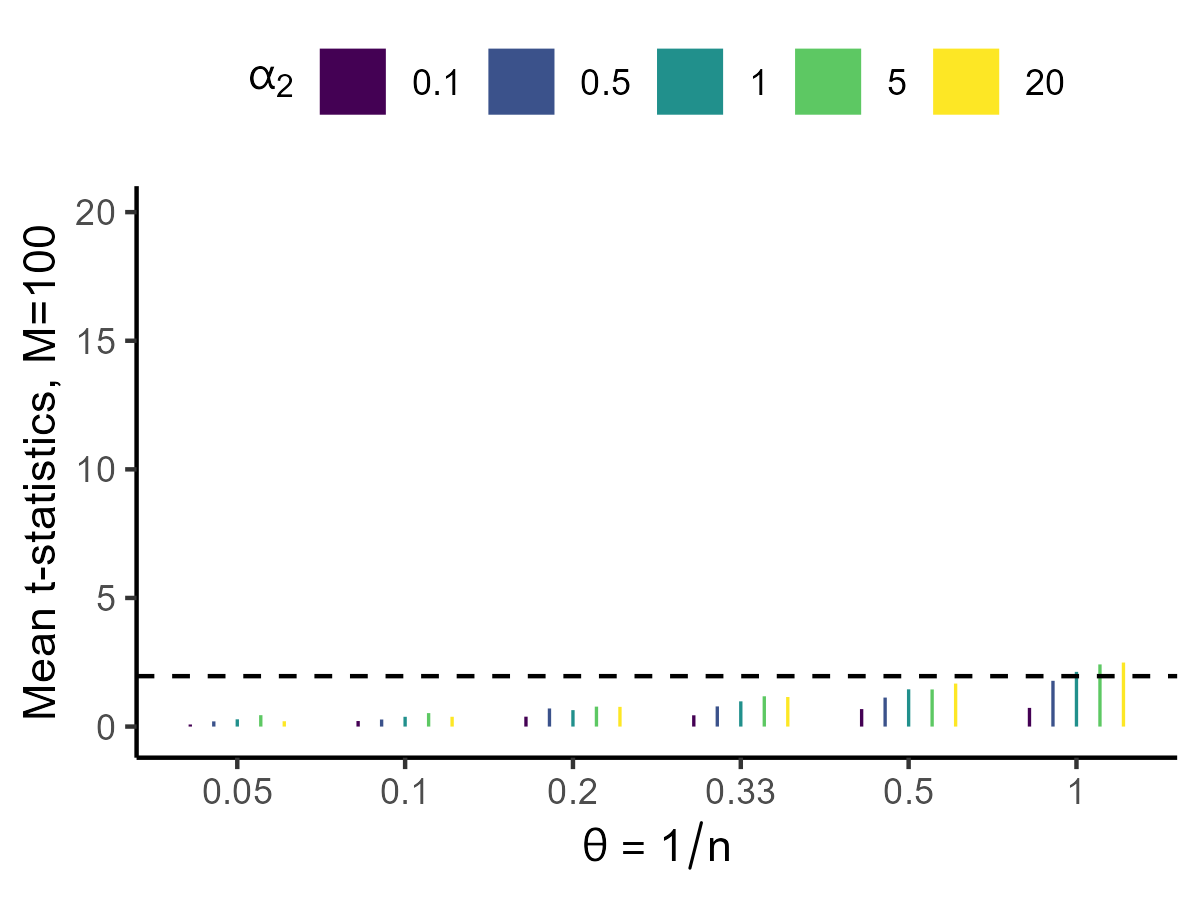
\includegraphics[width = 0.32\textwidth]
  {figuretable/theta_hat_t_statistics_100.png}}
  \subfloat[M=200]{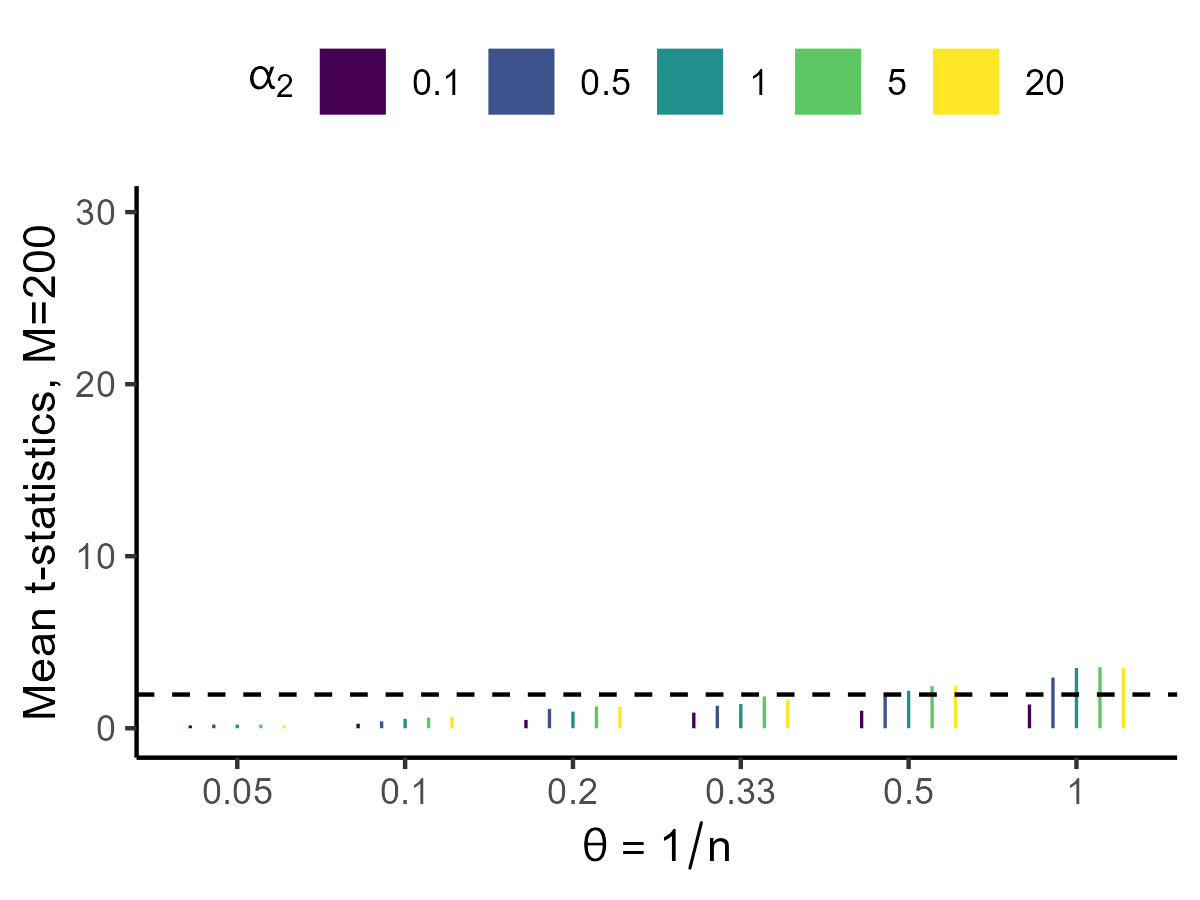
\includegraphics[width = 0.32\textwidth]
  {figuretable/theta_hat_t_statistics_200.png}}
  \subfloat[M=1000]{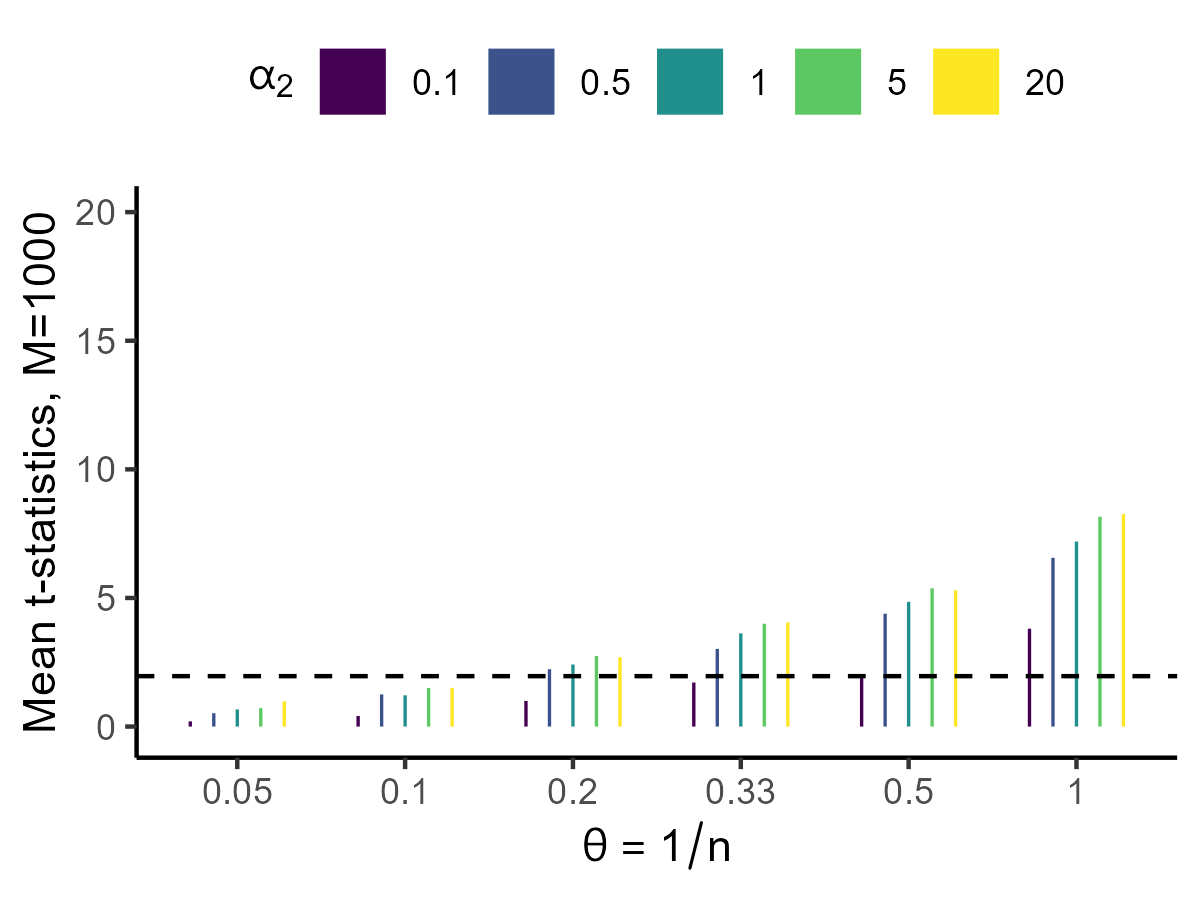
\includegraphics[width = 0.32\textwidth]
  {figuretable/theta_hat_t_statistics_1000.png}}\\
  \subfloat[M=2000]{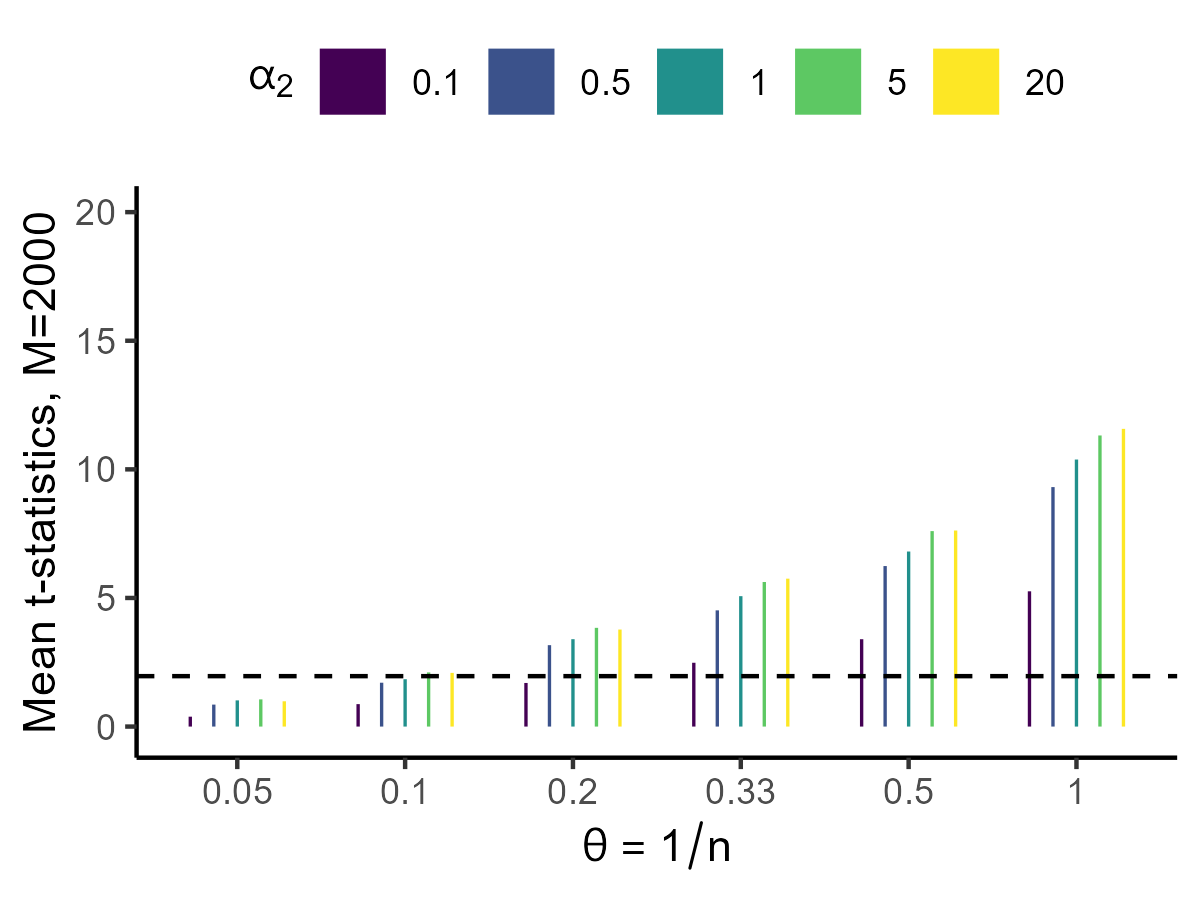
\includegraphics[width = 0.32\textwidth]
  {figuretable/theta_hat_t_statistics_2000.png}}
  \subfloat[M=5000]{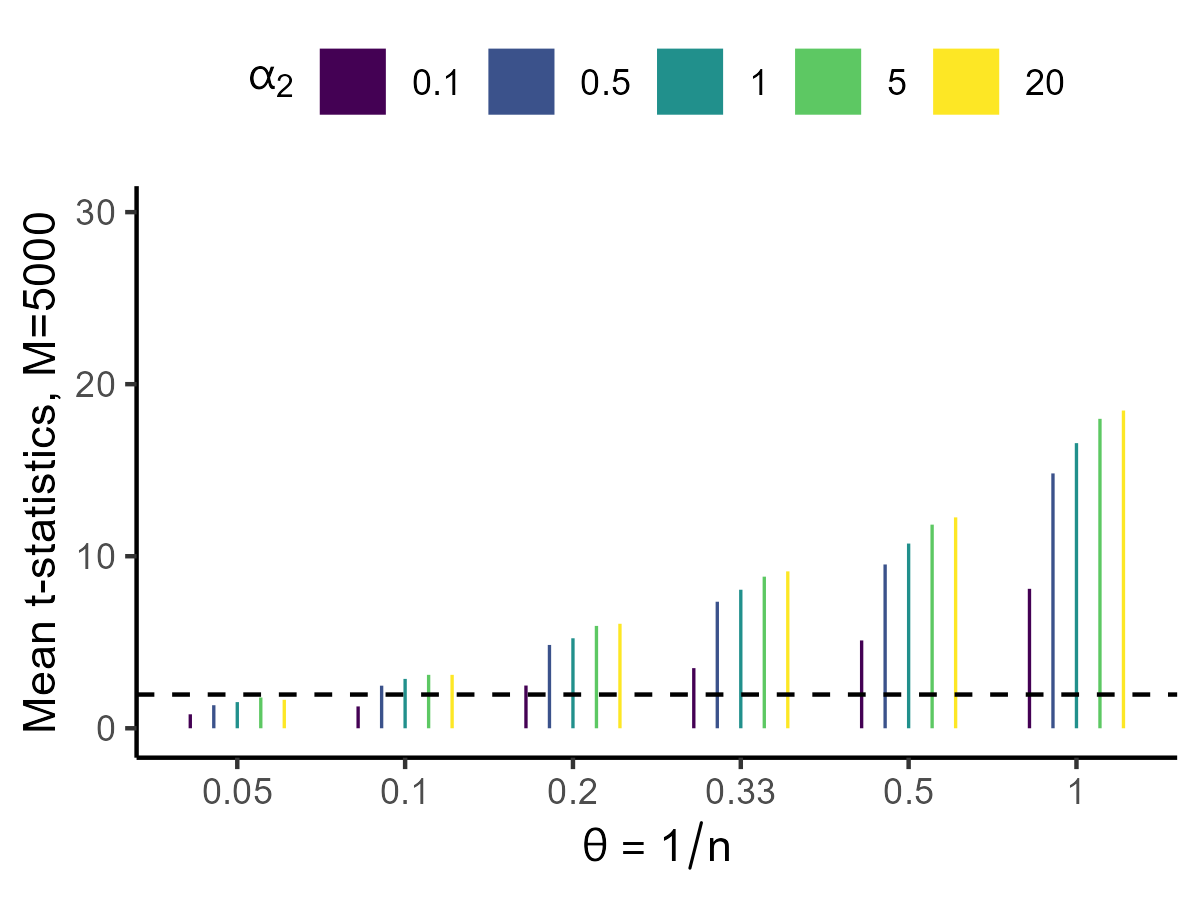
\includegraphics[width = 0.32\textwidth]
  {figuretable/theta_hat_t_statistics_5000.png}}
  \caption{Mean t-statistics of conduct parameter $\theta$}
  \label{fg:theta_hat_t_statistics}
  \end{center}
  \footnotesize
   Note: We simulate 100 datasets and calculate mean t-statistics of conduct parameter $\theta$.
\end{figure} 



\section{Conclusion}



\paragraph{Acknowledgments}
We thank Jeremy Fox and Isabelle Perrigne for their valuable advice. This research did not receive any specific grant from funding agencies in the public, commercial, or not-for-profit sectors. 

\newpage


\bibliographystyle{aer}
\bibliography{conduct_parameter}

\newpage

\setcounter{page}{1}
\appendix
\section{Online appendix}\label{sec:appendix}


\subsection{Simulation and estimation procedure}

We set true parameters and distributions as shown in Table \ref{tb:parameter_setting}. 
We follow the setting of PS. For simulation, we generate 1,000 data sets.
We separately estimate the demand and supply equation by using two-stage least squares (2SLS) estimation.
The instrumental variables for demand estimation are $Z^{d}_{t} = (Z^{R}_{t}, Y_t, H_{t}, K_{t})$ and the instrumental variables for supply estimation are $Z^{c}_{t} = (Z^{R}_{t}, W_{t}, R_{t}, Y_t)$. 

\begin{table}[!htbp]
    \caption{True parameters and distributions}
    \label{tb:parameter_setting}
    \begin{center}
    \subfloat[Parameters]{
    \begin{tabular}{cr}
            \hline
            & linear  \\
            $\alpha_0$ & $10.0$  \\
            $\alpha_1$ & $1.0$  \\
            $\alpha_2$ & $1.0$ \\
            $\alpha_3$ & $1.0$  \\
            $\gamma_0$ & $1.0$ \\
            $\gamma_1$ & $1.0$  \\
            $\gamma_2$ & $1.0$ \\
            $\gamma_3$ & $1.0$\\
            $\theta$ & $0.5$ \\
            \hline
        \end{tabular}
    }
    \subfloat[Distributions]{
    \begin{tabular}{crr}
            \hline
            & linear\\
            Demand shifter&  \\
            $Y_t$ & $N(0,1)$  \\
            Demand rotation instrument&   \\
            $Z^{R}_{t}$ & $N(10,1)$ \\
            Cost shifter&    \\
            $W_{t}$ & $N(3,1)$  \\
            $R_{t}$ & $N(0,1)$   \\
            $H_{t}$ & $W_{t}+N(0,1)$  \\
            $K_{t}$ & $R_{t}+N(0,1)$   \\
            Error&  &  \\
            $\varepsilon^{d}_{t}$ & $N(0,\sigma)$  \\
            $\varepsilon^{c}_{t}$ & $N(0,\sigma)$ \\
            \hline
        \end{tabular}
    }
    \end{center}
    \footnotesize
    Note: $\sigma=\{0.001, 0.5, 2.0\}$. $N:$ Normal distribution. $U:$ Uniform distribution.
\end{table}

\subsection{Details for our simulation settings}

To generate the simulation data, for each model, we first generate the exogenous variables $Y_t, Z^{R}_{t}, W_t, R_{t}, H_t$, and $K_t$ and the error terms $\varepsilon_{t}^c$ and $\varepsilon_{t}^d$ based on the data generation process in Table \ref{tb:parameter_setting}.
We compute the equilibrium quantity $Q_{t}$ for the linear model by \eqref{eq:quantity_linear}.
We then compute the equilibrium price $P_t$ by substituting $Q_{t}$ and other variables into the demand function \eqref{eq:linear_demand}.

We estimate the equations using the \texttt{ivreg} package in \texttt{R}.
An important feature of the model is that we have an interaction term of the endogenous variable $Q_{t}$ and the instrumental variable $Z^{R}_{t}$.
The \texttt{ivreg} package automatically detects that the endogenous variables are $Q_{t}$ and the interaction term $Z^{R}_{t}Q_{t}$, running the first stage regression for each endogenous variable with the same instruments. To confirm this, we manually write R code to implement the 2SLS model. 
When the first stage includes only the regression of $Q_{t}$, estimation results from our code differ from the results from \texttt{ivreg}. 
However, when we modify the code to regress $Z^{R}_{t}Q_{t}$ on the instrument variables and estimate the second stage by using the predicted values of $Q_{t}$ and $Z^{R}_{t}Q_{t}$, the result from our code and the result from \texttt{ivreg} coincide.


\subsection{Other experiments}

\begin{table}[!htbp]
    \caption{Estimation results in Table 2 of from PS}
    \label{tb:linear_linear_sigma_Perloff_Shen}
    \begin{center}
        \begin{tabular}{cllll}
            \hline
            & $\sigma=0.001$ & $\sigma=0.5$ & $\sigma=1$ & $\sigma=2$ \\
            $\alpha_0$ & $10.00\ (0.001)$ & $9.96\ (0.33)$ & $9.86\ (0.65)$ & $9.46 (1.20)$ \\
            $\alpha_1$ & $1.00\ (0.004)$ & $0.99\ (1.98)$ & $0.97\ (3.96)$ & $0.88 (7.80)$ \\
            $\alpha_2$ & $1.00\ (0.004)$ & $0.99\ (0.21)$ & $0.97\ (0.42)$ & $0.87\ (0.82)$ \\
            $\gamma_1$ & $0.46\ (0.88)$ & $0.46\ (0.91)$ & $0.47\ (0.93)$ & $0.49\ (1.04)$ \\
            $\gamma_2$ & $5.85\ (7.89)$ & $5.85\ (8.15)$ & $5.78\ (8.21)$ & $5.73\ (8.66)$ \\
            $\theta$ & $-0.31\ (1.31)$ & $-0.29\ (1.34)$ & $0.09\ (11.48)$ & $-1.53\ (30.41)$ \\
            \hline
        \end{tabular}
    \end{center}\footnotesize
    Note: True parameters: $\alpha_1 = \alpha_2 = \gamma_0 = \gamma_1 = \gamma_2  = \gamma_3 = 1, \alpha_0 = 10, \alpha_3 = 0,$ and $\theta = 0.5$. PS exclude $Y_t$. We change the parameter notations from the original study. Note that PS do not provide $\gamma_0$ and $\gamma_3$.
\end{table}

First, we replicate the result in PS. For comparison, we report the means and standard deviations (SDs).
To replicate the result, we exclude the demand shifter $Y_t$ and assume the coefficient $\alpha_3$ of $Y_t$ is zero, indicating that there is no demand shifter for supply estimation.
For reference, Table \ref{tb:linear_linear_sigma_Perloff_Shen} is quoted from PS, although we modify some notation.
Sample size in each simulation dataset is 50 and the table shows the means and SDs of the 2SLS estimators from 1,000 simulations.
It shows that demand estimation becomes more accurate as the values of the SDs of the error terms, that is, $\sigma$ decreases.
In contrast, supply estimation is still biased and the SD of the conduct parameter becomes larger as the value of $\sigma$ increases.

Our replication results are presented in Table \ref{tb:linear_linear_sigma_1_without_demand_shifter_y}.
Each panel presents the simulation results under different SDs.
This result uses the same data generation process as PS. 
To determine whether we can correctly replicate the result in PS, we focus on the first two columns in each panel.
These two columns show the means and SDs of the simulation results when sample size is 50.
While demand parameters can be accurately estimated, although the value of $\sigma$ becomes higher, the supply parameters are biased.
In particular, when $\sigma$ is large and sample size is small, the SDs of the parameters in supply equation become large.
Thus, we reveal the patterns in PS that do not provide any details.

As PS fix sample size to 50, we also examine the effect of changing sample size.
As expected, increasing sample size given a value of $\sigma$ decreases the SDs of supply parameters.
However, no simulation result is close to the true values of supply parameters as well as the conduct parameter.
These results are consistent with PS.

\begin{table}[!htbp]
  \begin{center}
      \caption{Estimation results of the linear model without demand shifter}
      \label{tb:linear_linear_sigma_1_without_demand_shifter_y} 
      \subfloat[$\sigma=0.001$]{
\begin{tabular}[t]{lrrrrrrrr}
\toprule
  & (1) $n=50$ / Mean & (1) $n=50$ / SD & (2) $n=100$ / Mean & (2) $n=100$ / SD & (3) $n=200$ / Mean & (3) $n=200$ / SD & (4) $n=1000$ / Mean & (4) $n=1000$ / SD\\
\midrule
$\alpha_{0}$ & 10.000 & 0.0009 & 10.000 & 0.0006 & 10.000 & 0.0004 & 10.000 & 0.0002\\
$\alpha_{1}$ & 1.000 & 0.004 & 1.000 & 0.003 & 1.000 & 0.002 & 1.000 & 0.0009\\
$\alpha_{2}$ & 1.000 & 0.0005 & 1.000 & 0.0003 & 1.000 & 0.0002 & 1.000 & 0.0001\\
$\gamma_{0}$ & 5.446 & 6.981 & 5.388 & 7.986 & 5.423 & 7.825 & 5.063 & 6.801\\
$\gamma_{1}$ & 0.506 & 0.775 & 0.512 & 0.888 & 0.509 & 0.869 & 0.549 & 0.756\\
$\gamma_{2}$ & 0.506 & 0.776 & 0.512 & 0.887 & 0.509 & 0.869 & 0.549 & 0.756\\
$\theta$ & -0.241 & 1.164 & -0.231 & 1.331 & -0.237 & 1.304 & -0.177 & 1.134\\
$R^{2}$ (demand) & 1.000 & 0.0000004 & 1.000 & 0.0000003 & 1.000 & 0.0000002 & 1.000 & 8e-08\\
$R^{2}$ (supply) & 1.000 & 0.000008 & 1.000 & 0.00001 & 1.000 & 0.00001 & 1.000 & 0.000008\\
Sample size ($T$) &  & 50 &  & 100 &  & 200 &  & 1000\\
\bottomrule
\end{tabular}
}\\
      \subfloat[$\sigma=0.5$]{
\begin{tabular}[t]{lrrrrrrrr}
\toprule
  & (1) $n=50$ / Mean & (1) $n=50$ / SD & (2) $n=100$ / Mean & (2) $n=100$ / SD & (3) $n=200$ / Mean & (3) $n=200$ / SD & (4) $n=1000$ / Mean & (4) $n=1000$ / SD\\
\midrule
$\alpha_{0}$ & 9.993 & 0.466 & 9.993 & 0.312 & 10.001 & 0.215 & 10.002 & 0.093\\
$\alpha_{1}$ & 0.963 & 2.138 & 0.965 & 1.484 & 1.012 & 1.023 & 0.991 & 0.441\\
$\alpha_{2}$ & 1.002 & 0.243 & 1.002 & 0.168 & 0.999 & 0.118 & 1.002 & 0.049\\
$\gamma_{0}$ & 5.332 & 10.459 & 5.227 & 11.592 & 5.112 & 15.871 & 5.470 & 7.476\\
$\gamma_{1}$ & 0.405 & 3.214 & 0.434 & 1.989 & 0.474 & 1.744 & 0.516 & 1.102\\
$\gamma_{2}$ & 0.517 & 1.157 & 0.528 & 1.222 & 0.546 & 1.816 & 0.504 & 0.830\\
$\theta$ & -0.210 & 1.879 & -0.206 & 1.951 & -0.186 & 2.705 & -0.247 & 1.238\\
$R^{2}$ (demand) & 0.720 & 0.088 & 0.725 & 0.061 & 0.726 & 0.041 & 0.728 & 0.018\\
$R^{2}$ (supply) & 0.160 & 7.674 & -0.119 & 19.529 & -0.724 & 30.775 & 0.491 & 2.041\\
Sample size (n) &  & 50 &  & 100 &  & 200 &  & 1000\\
\bottomrule
\end{tabular}
}\\
  \end{center}\footnotesize
  Note: True parameters: $\alpha_1 = \alpha_2 =  \gamma_0 = \gamma_1 = \gamma_2  =  1, \alpha_0 = 10, \theta = 0.5.$ and $\alpha_3 =0$. For comparison, we report the mean and SD.
\end{table} 

\begin{table}[!htbp]
  \ContinuedFloat
  \begin{center}
      \caption{Estimation results of the linear model without demand shifter (Continued)}
      \subfloat[$\sigma=1.0$]{
\begin{tabular}[t]{lrrrrrrrr}
\toprule
  & Mean & SD & Mean  & SD  & Mean   & SD   & Mean    & SD   \\
\midrule
$\alpha_{0}$ & 9.975 & 0.964 & 9.953 & 0.636 & 10.007 & 0.441 & 9.991 & 0.189\\
$\alpha_{1}$ & 1.120 & 4.491 & 0.942 & 2.885 & 0.883 & 2.055 & 1.035 & 0.902\\
$\alpha_{2}$ & 0.981 & 0.492 & 0.993 & 0.326 & 1.015 & 0.227 & 0.993 & 0.101\\
$\gamma_{0}$ & 5.631 & 9.410 & 5.520 & 7.580 & 5.161 & 9.226 & 5.556 & 7.424\\
$\gamma_{1}$ & -0.107 & 19.285 & 0.129 & 5.240 & 0.488 & 3.541 & 0.489 & 1.210\\
$\gamma_{2}$ & 0.476 & 1.043 & 0.495 & 0.835 & 0.540 & 1.030 & 0.494 & 0.820\\
$\theta$ & -0.201 & 3.603 & -0.217 & 1.478 & -0.183 & 1.528 & -0.260 & 1.229\\
$R^{2}$ (demand) & 0.205 & 0.357 & 0.234 & 0.221 & 0.232 & 0.150 & 0.245 & 0.060\\
$R^{2}$ (supply) & -0.920 & 17.898 & -0.395 & 5.271 & -0.904 & 12.486 & -0.421 & 12.047\\
Sample size (n) &  & 50 &  & 100 &  & 200 &  & 1000\\
\bottomrule
\end{tabular}
}\\
    \subfloat[$\sigma=2.0$]{
\begin{tabular}[t]{lrrrrrrrr}
\toprule
  & Mean & SD & Mean  & SD  & Mean   & SD   & Mean    & SD   \\
\midrule
$\alpha_{0}$ & 9.515 & 6.752 & 9.912 & 1.479 & 9.987 & 0.943 & 9.987 & 0.396\\
$\alpha_{1}$ & 0.362 & 19.344 & 0.710 & 6.192 & 1.154 & 4.363 & 0.986 & 1.728\\
$\alpha_{2}$ & 0.934 & 1.092 & 1.004 & 0.743 & 0.981 & 0.494 & 0.998 & 0.204\\
$\gamma_{0}$ & 5.658 & 6.892 & 5.464 & 8.387 & 5.695 & 8.243 & 5.572 & 10.796\\
$\gamma_{1}$ & 0.956 & 52.166 & 1.715 & 42.062 & -0.056 & 11.467 & 0.388 & 3.140\\
$\gamma_{2}$ & 0.479 & 0.827 & 0.496 & 0.907 & 0.486 & 0.902 & 0.497 & 1.185\\
$\theta$ & -0.296 & 5.941 & -0.439 & 5.106 & -0.235 & 2.034 & -0.256 & 1.771\\
$R^{2}$ (demand) & -3.456 & 87.362 & -0.513 & 1.557 & -0.436 & 0.563 & -0.376 & 0.185\\
$R^{2}$ (supply) & -1.104 & 5.881 & -2.311 & 26.606 & -1.993 & 26.973 & -3.591 & 49.060\\
Sample size ($T$) &  & 50 &  & 100 &  & 200 &  & 1000\\
\bottomrule
\end{tabular}
}
  \end{center}\footnotesize
  Note: True parameters: $\alpha_1 = \alpha_2 =  \gamma_0 = \gamma_1 = \gamma_2  =  1, \alpha_0 = 10, \theta = 0.5.$ and $\alpha_3 =0$. For comparison, we report the mean and SD.
\end{table} 



\end{document}